\sectionbreak \section{ \standartTitleFont
  Введение
}

\subsection{ \standartTitleFont
  Назначения проекта и требования к нему
}

{\standartFont

  \par Модуль DataManipulator предназначен для различного рода обработки данных, с целью получения наборов данных (датасетов) необходимых для обучения моделей неройнных сетей. DataManipulator помогает преодолеть этап анализа и обработки данных, а также этап конструирования признаков.

  \par
}

\subsection{ \standartTitleFont
  Введение в предметную область
}

{\standartFont

  \par Модуль DataManipulator предназначен для различного рода обработки данных, с целью получения наборов данных (датасетов) необходимых для обучения моделей неройнных сетей. DataManipulator помогает преодолеть этап анализа и обработки данных, а также этап конструирования признаков.

  \par
}

\subsection{ \standartTitleFont
  Введение во временные ряды и прогнозирование
}

{\standartFont

  \par Одним из ключевых понятий данной работы является понятие временных рядов. Что же это? Временные ряды {--} это, по сути, некоторая последовательность, каждый элемент из которой состоит из двух или более параметров, а один из них обязательно должен обозначать время. Причём, все эти элементы в последовательности расположены в хронологическом порядке, то есть в порядке возрастания параметра времени.

  \par Параметр времени может быть представлен в разных форматах. Выбор формата времени зависит от задачи, удобства использования, длительности, в пределах которой будут собираться данные, а также от требуемой точности. Например, в случае если данные фиксируются раз в день, то хорошо подойдёт отсчёт времени по дням с указанием месяца и года. Если же данные фиксируются в определённые моменты дня, то к вышеописанному стоит прибавить указание часа и минуты фиксации. При необходимости можно указывать и секунды, и миллисекунды. Но что, если не особо-то и важно знать, в какой год, месяц или день это происходило, когда важно знать, сколько прошло времени от начала того или иного процесса? Тогда, скорее подойдёт формат дискретного времени. С помощью этого формата можно узнать длительность процесса в единственной выбранной нами единице измерения времени. Например, если сохранять время в секундах, то 1000-ча секунд сохранит свой формат 1000-чи секунд, время не будет переведено в 16-ать минут и 40-ок секунд. Всё это позволяет не привязываться к датам, которые не особо-то и влияют на технологический процесс промышленного оборудования.

  \par Остальные параметры могут уже характеризовать или описывать какой-либо процесс или какие-либо процессы, причём даже не обязательно одного элемента, а даже целой системы элементов. Так, например, когда элемент последовательности состоит из двух признаков, а один из которых, как уже известно, время, то второй, конечно же, уже будет обозначать характеристику или состояние изучаемого нами элемента. Но как только появляется три или более признаков, тогда уже можно говорить о фиксации характеристик или состояний разных элементов изучаемой системы в один и тот же момент времени или же о фиксации характеристики или состояния одного из множества элементов системы, но с указание этого элемента, например, с помощью идентификационного номера элемента. Как можно убедиться, временные ряды дают весьма гибкую возможность описания процессов или систем относительно времени.

  \par Технологический процесс пастеризационной установки как раз и представляет собой временной ряд, в котором имеется информация о показаниях различных датчиков в определённые моменты времени. Поэтому, говоря о данных технологического процесса пастеризационной установки, мы будем понимать, что они имеют форму временных рядов.

  \par А что из себя представляет работа с временными рядами? В основном работа делится на две части. Первая часть {--} это понимание структуры временного ряда, его закономерностей, таких как цикличность, тренд, сезонность и так далее, обработка данных временного ряда, визуализация данных, в общем, это всесторонний анализ временного ряда. Если опускать различные математические, статистические и тому подобные подробности, то анализ также может дать нам возможность понять, как начинался процесс, как шёл, развивался и на чём он закончился или остановился на данном моменте времени.  Строго говоря, нейронным сетям, как и исследователям временных рядов, тоже необходимо это понять, чтобы выполнить вторую часть работы, а именно, составление прогноза, что, зачастую, и является основной задачей работы с временным рядом. Да, анализ данных временного ряда технологического процесса делается с целью понять, что будет происходить с этим процессом дальше. Но чем нам так полезна информация о будущем, зачем она нужна? Для этого необходимо понять, что есть прогноз.

  \par Сам прогноз {--} это некоторая случайная величина, характеризующая вероятность того, что график в будущем пройдёт через определённую точку или некоторую область. Тогда прогнозирование {--} это получение максимально точных прогнозов, или, если говорить в отрыве от понятия прогноза, то это точное предсказание будущего, учитывающее исторические данные об объекте прогнозирования, а также знания о любых будущих событиях, которые могут повлиять на прогнозы.

  \par Как понять, что прогнозы действительные? Прогнозы являются таковыми, если они отражают подлинные закономерности и взаимосвязи, которые есть в исторических данных, при этом не повторяя прошлые события, которые более не актуальны или уже не повторяются.

  \par Что необходимо, чтобы составить хороший прогноз на основе временных рядов? Для этого обычно требуется выполнить следующие шаги:

  \par 1. Определить задачу.
  \par 2. Собрать информацию.
  \par 3. Произвести предварительный анализ.
  \par 4. Выбрать и создать модель прогнозирования.
  \par 5. Использовать и оценить модель прогнозирования.

  \par Вкратце разберём каждый пункт. При определении задачи необходимо понять, что вообще будет прогнозироваться, как будут использоваться прогнозы, благодаря чему будут получены прогнозы, кому эти прогнозы нужны или для чего. Второй пункт подразумевает непосредственный сбор или получение данных, а также оценка накопленного опыта людей, которые собирают данные и используют прогнозы. Для выполнения третьего пункта необходимо визуализировать данные, составить инфографику, если она необходима, определить взаимосвязь с признаками, закономерности временных рядов, качество данных и так далее, другими словами, провести анализ данных. На четвёртом пункте необходимо либо приобрести и адаптировать готовую модель, либо создать её самостоятельно. Но модель должна учитывать исторические данные, силы взаимосвязи между прогнозируемым признаком и любым другим признаком, а также способы использования прогнозов. В заключении проводится тестирование, оценивание, развёртывание и сопровождение модели прогнозирования.

  \par

}

\subsection{ \standartTitleFont
  Анализ имеющихся данных 
}


{\standartFont

  \par Модуль DataManipulator предназначен для различного рода обработки данных, с целью получения наборов данных (датасетов) необходимых для обучения моделей неройнных сетей. DataManipulator помогает преодолеть этап анализа и обработки данных, а также этап конструирования признаков.

  \par

  \begin{sidewaysfigure}
    \centering
    \def\svgwidth{\textwidth}
    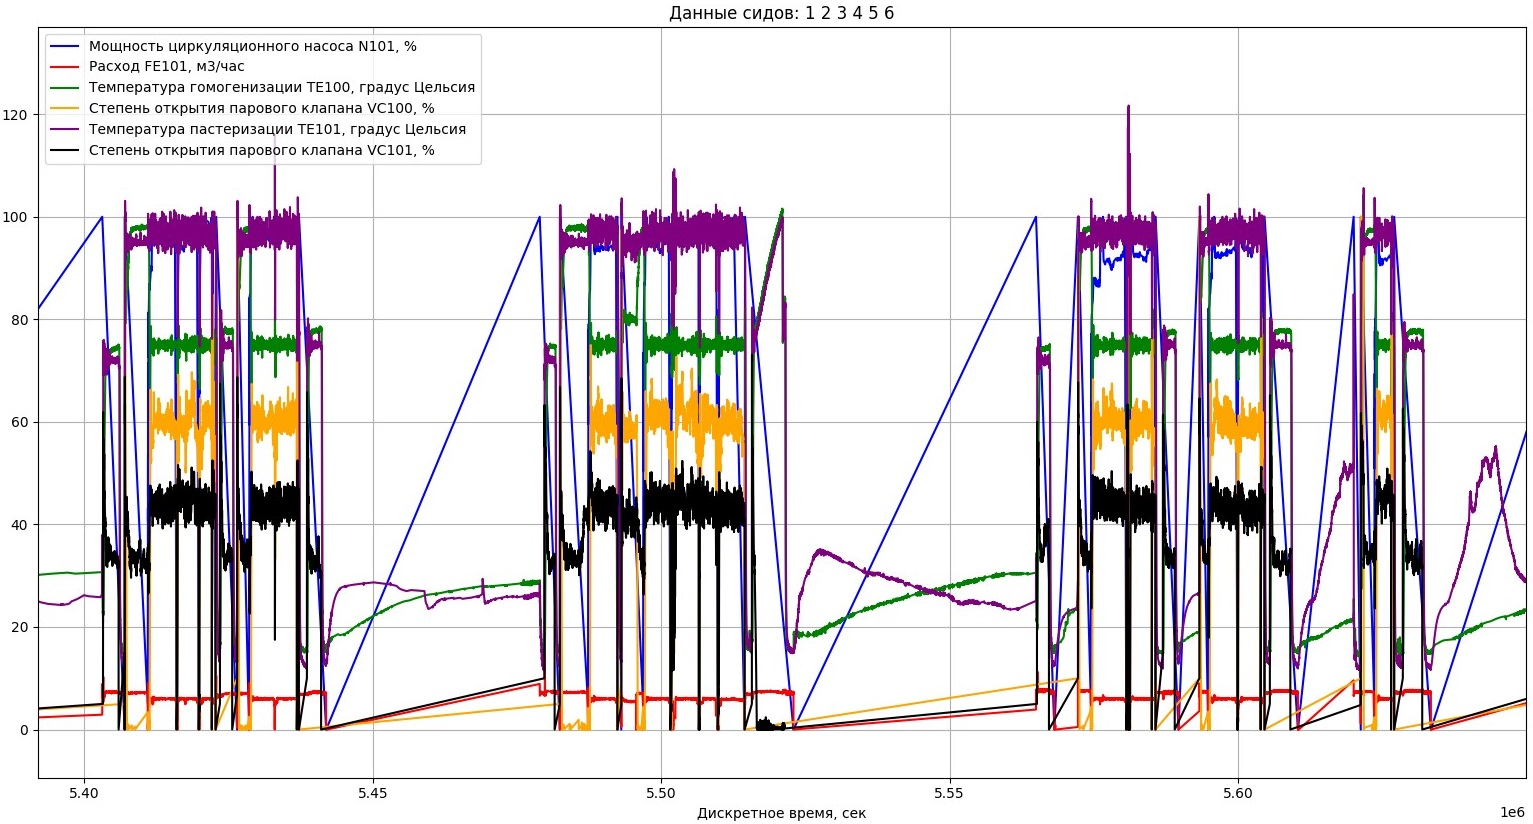
\includegraphics[scale=0.6]{images/forGeneral/data_1_visual.jpg}
    \caption{Визуализация данных 1-ого файла}
    \label{fig:Data1Visual}
  \end{sidewaysfigure} 

  \begin{sidewaysfigure}
    \centering
    \def\svgwidth{\textwidth}
    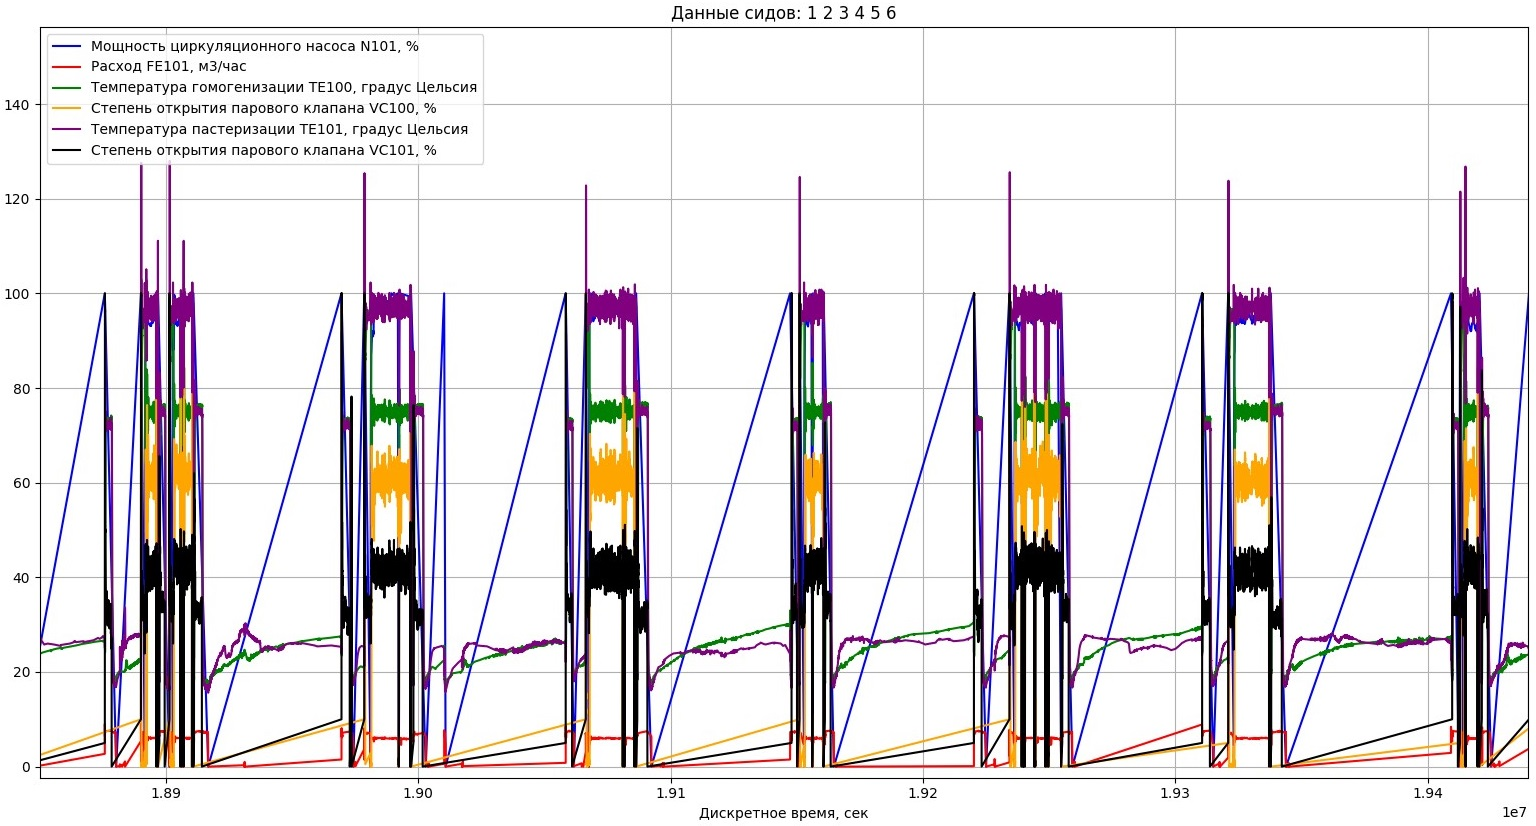
\includegraphics[scale=0.6]{images/forGeneral/data_2_visual.jpg}
    \caption{ Визуализация данных 2-ого файла с растянутым масштабом по оси абсцисс}
    \label{fig:Data2Visual}
  \end{sidewaysfigure} 

  \begin{sidewaysfigure}
    \centering
    \def\svgwidth{\textwidth}
    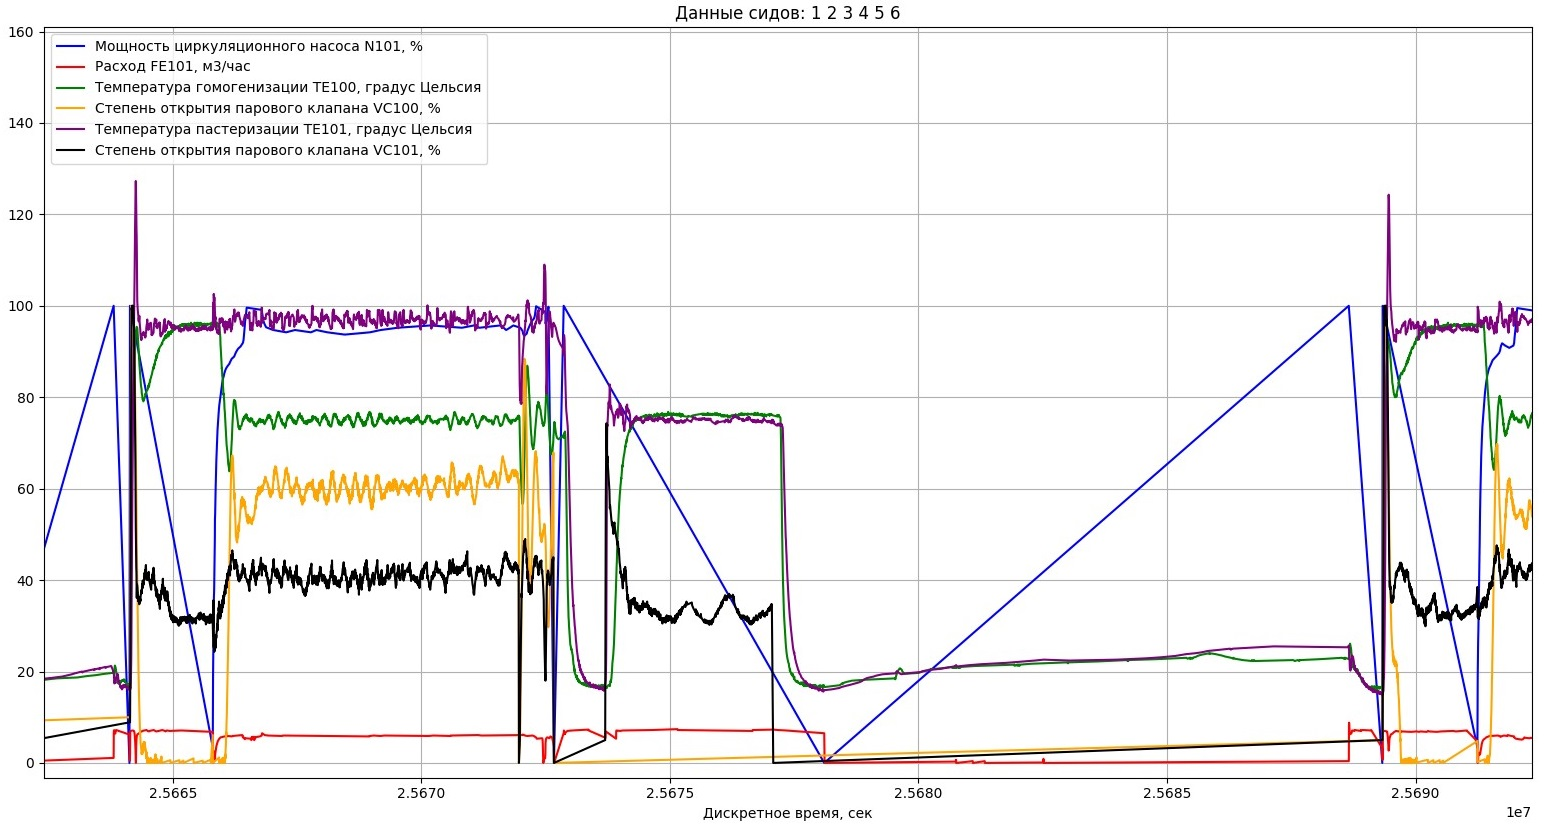
\includegraphics[scale=0.6]{images/forGeneral/data_3_visual.jpg}
    \caption{ Визуализация данных 3-ого файла с cуженным масштабом по оси абсцисс}
    \label{fig:Data3Visual}
  \end{sidewaysfigure} 

}